\documentclass{beamer}
\usetheme{tokitex}

\usepackage{graphics}
\usepackage{multirow}
\usepackage{tabto}

\usepackage[english,bahasa]{babel}
\newtranslation[to=bahasa]{Section}{Bagian}
\newtranslation[to=bahasa]{Subsection}{Subbagian}

\usepackage{listings, lstautogobble}
\usepackage{color}

\definecolor{dkgreen}{rgb}{0,0.6,0}
\definecolor{gray}{rgb}{0.5,0.5,0.5}
\definecolor{mauve}{rgb}{0.58,0,0.82}

\lstset{frame=tb,
  language=pascal,
  aboveskip=1mm,
  belowskip=1mm,
  showstringspaces=false,
  columns=fullflexible,
  keepspaces=true,
  basicstyle={\small\ttfamily},
  numbers=none,
  numberstyle=\tiny\color{gray},
  keywordstyle=\color{blue},
  commentstyle=\color{dkgreen},
  stringstyle=\color{mauve},
  breaklines=true,
  breakatwhitespace=true,
  autogobble=true
}

\title{Perkenalan Graph}
\author{Tim Olimpiade Komputer Indonesia}
\date{}

\lstset{escapeinside={<@}{@>},belowskip=\baselineskip}
\definecolor{mygreen}{rgb}{0, 0.597, 0.199}

\begin{document}

\begin{frame}
\titlepage
\end{frame}

\begin{frame}
\frametitle{Pendahuluan}
Melalui dokumen ini, kalian akan:
\begin{itemize}
	\item Mengenal konsep dan terminologi graph
	\item Mengetahui jenis-jenis graph
	\item Mengenal representasi graph pada pemrograman
	\item Mengenal metode-metode yang digunakan dalam graph
\end{itemize}

\end{frame}

\begin{frame}
\frametitle{Mengenal Graph}
Graph merupakan struktur data yang terdiri dari \alert{node/vertex} dan \alert{edge}. Node direpresentasikan dengan bentuk lingkaran dan edge direpresentasikan dengan bentuk garis pada ilustrasi dibawah ini.

\begin{figure}
	\centering
	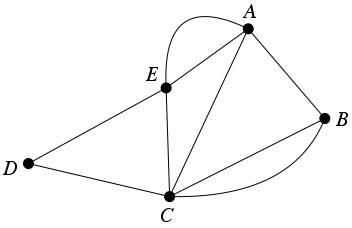
\includegraphics[width=6 cm]{asset/graph.jpg}
\end{figure}
\end{frame}

\begin{frame}
\frametitle{Mengenal Graph (lanj.)}
Melalui ilustrasi diatas, dapat disimpulkan bahwa edge memiliki fungsi untuk menghubungkan antar-node. \alert{Degree} sebuah node didefinisikan sebagai jumlah edge yang terhubung pada node tersebut.\newline\newline
Pada contoh graph di atas, maka degree node A adalah 4, degree node B adalah 3, dan seterusnya. Degree node dalam graph bisa berapa saja, tidak seperti binary search tree yang pasti hanya dapat memiliki maksimal 2 anak dan 1 parent. 
\end{frame}

\begin{frame}
\frametitle{Jenis-jenis Graph}
Berdasarkan hubungan antar node, graph terbagi menjadi 2:
\begin{itemize}
	\item Directed graph, yaitu graph satu arah. Di graph jenis ini, jika terdapat edge dari A ke B, maka belum tentu terdapat edge dari B ke A. Contoh graph ini adalah kota-kota sebagai nodenya dan jalan 1 arah sebagai edgenya.
	\item Undirected graph, yaitu graph dua arah. Dalam graph ini, jika terdapat edge dari A ke B, maka pasti juga terdapat edge dari B ke A. Contoh graph jenis ini adalah kota-kota sebagai nodenya dan jalan 2 arah sebagai edgenya.
\end{itemize}
\end{frame}

\begin{frame}
\frametitle{Jenis-jenis Graph (lanj.)}
Berdasarkan bobot dari edgenya, graph juga terbagi menjadi 2:
\begin{itemize}
	\item Unweighted Graph, yaitu graph yang mana edgenya tidak memiliki value, sehingga semua edge memiliki weight 1 dan hanya bermakna bahwa memang terdapat hubungan antar node yang dihubungkannya.
	\item Weighted Graph, yaitu graph yang mana edgenya memiliki bobot yang berbeda-beda. Bobot pada edge ini seringkali berupa biaya atau jarak yang harus ditempuh jika menggunakan edge tersebut.
\end{itemize}
\end{frame}

\begin{frame}
\frametitle{Representasi Graph pada Pemrograman}

Graph biasanya direpesentasikan dalam pemrograman menggunakan 2 metode, yaitu adjacency matrix dan adjacency list. Masing-masing representasi memiliki keuntungan dan kerugiannya masing-masing. Oleh karena itu, penggunaan representasi graph sangat bergantung dengan masalah yang sedang kita hadapi.
\end{frame}

\begin{frame}
\frametitle{Adjacency Matrix}

Pada adjacency matrix, kita harus menyediakan array 2 dimensi dengan ukuran N x N yang mana N merupakan banyaknya node/vertex. \newline\newline
Awalnya, seluruh elemen matrix berisi nilai 0 yang menandakan bahwa tidak terdapat edge. Pada unweighted graph, jika terdapat edge dari node A ke node B, maka kita ganti isi dari $matrix[A][B] = 1$. Misal pada weighted graph dan terdapat edge dari A ke B dengan bobot C, maka update $matrix[A][B] = C$.
\end{frame}

\begin{frame}
\frametitle{Adjacency List}

Pada adjacency list, graph disimpan dalam array of lists. Tiap list berisi keterangan mengenai edge yang terdapat dalam suatu node. Ukuran dari array merupakan N yang mana N merupaka banyaknya node/vertex. \newline\newline
Awalnya, seluruh list tidak memiliki isi yang menandakan bahwa belum terdapat edge dalam graph tersebut. Pada unweighted graph, jika terdapat edge dari node A ke node B, maka, masukkan B kedalam list A. Pada weighted graph, jika terdapat edge dari node A ke node B dengan bobot C, maka masukkan \{B,C\} kedalam list A. Di sini isi dari list terdapat 2 item, yaitu node yang dituju beserta bobotnya
\end{frame}


\begin{frame}[fragile]
\frametitle{Pseudocode Representasi Graph}

Adjacency Matrix
\begin{lstlisting}
	integer AdjMatrix[N][N]
	set AdjMatrix = 0
	
	<@\textcolor{mygreen}{//edge dari 1 ke 4 pada undirected unweighted graph}@>
	AdjMatrix[1][4] = 1
	AdjMatrix[4][1] = 1
\end{lstlisting}
Adjacency List
\begin{lstlisting}
	List<integer> AdjList[N]
	
	<@\textcolor{mygreen}{//edge dari 1 ke 4 pada undirected unweighted graph}@>
	AdjList[1].push(4)
	AdjList[4].push(1)
	
\end{lstlisting}
\end{frame}

\begin{frame}
\frametitle{Keuntungan dan Kerugian Representasi Graph}

\begin{itemize}
	\item Adjacency Matrix memakan lebih banyak memori. Hal ini dikarenakan adjacency matrix menyimpan keterangan dari satu node ke semua node. Sedangkan dalam adjacency list, suatu node hanya menyimpan keterangan mengenai node lain yang memiliki edge. Oleh karena itu, adjacency list lebih baik digunakan ketika edge yang terdapat tidak teralu banyak.
	\item Untuk melakukan pengecekan atau perubahan edge dari A ke B, pada adjacency matrix dapat dilakukan dengan hanya melihat dan mengubah matrix[A][B]. Sedangkan pada adjacency list, kita harus mengiterasi seluruh elemen pada list[A]
\end{itemize}
\end{frame}

\begin{frame}
\frametitle{Keuntungan dan Kerugian Representasi Graph (lanj.)}
\begin{itemize}
	\item Jika ada edge dari A ke B yang akan dibuang, maka pada adjacency matrix kita hanya perlu mengubah nilai Matrix[A][B]. Sedangkan pada adjacency list, harus dilakukan iterasi terlebih dahulu untuk mencari edge tersebut, lalu menghapusnya juga lebih rumit karena harus menggeser seluruh elemen setelahnya.
	\item Untuk mencari tetangga-tetangganya, maka pada adjacency matrix perlu dilakukan iterasi terhadap seluruh node yagn ada. Sementara itu, pada adjacency list hanya perlu dilakukan iterasi pada list yang isinya merupakan tetangga dari node yang bersangkutan.
\end{itemize}
\end{frame}

\begin{frame}
\frametitle{Graph Traversal}

Sekarang kita telah mengetahui bagaimana cara menyimpan graph dalam pemrograman. Namun, representasi tersebut belum berguna karena kita belum dapat mencari informasi dari representasi tersebut.\newline\newline
Kali ini kita akan belajar mengenai \alert{Graph Traversal}, yaitu penelusuran pada graph. Misalkan kita diberikan suatu graph. Lalu, kita ditanya apakah dari node A bisa pergi ke node B menggunakan edge yang ada? Untuk mendapatkan jawabannya, kita tentu harus menelusuri graph tersebut dari node A.\newline\newline
Terdapat 2 metode yang digunakan untuk menelusuri graph, yaitu BFS dan DFS.
\end{frame}

\begin{frame}
\frametitle{DFS}

\alert{DFS} merupakan singkatan dari Depth-First Search. Berdasarkan namanya, dapat disimpulkan bahwa DFS akan mencari node-node yang lebih dalam(depth-first) terlebih dahulu. Sebagai contoh misal terdapat graph seperti berikut

\begin{figure}
	\centering
	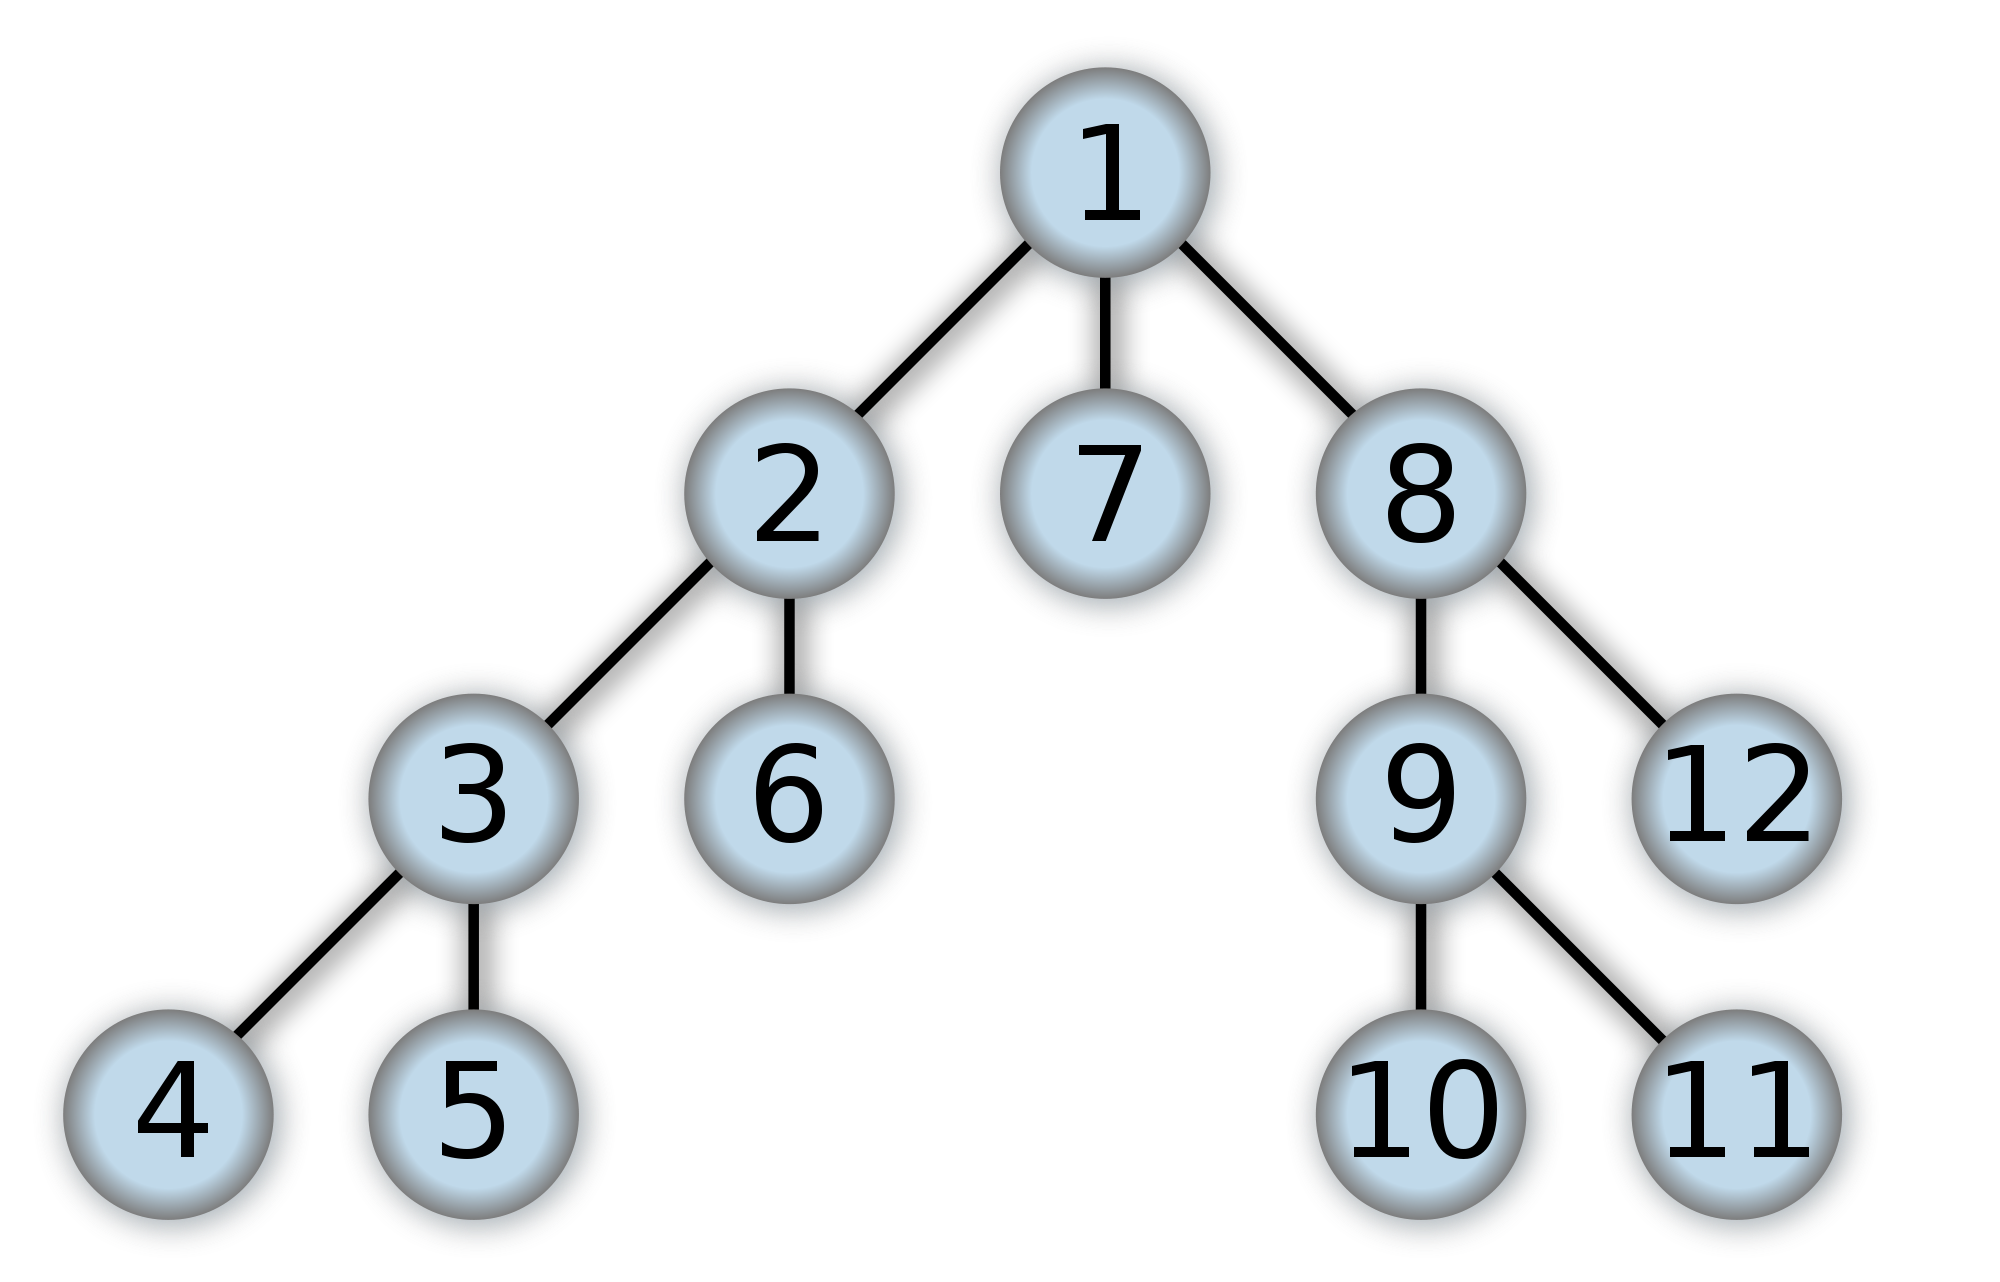
\includegraphics[width=6 cm]{asset/dfs.png}
\end{figure}
\end{frame}

\begin{frame}
\frametitle{DFS (lanj.)}
Dalam gambar di atas, angka menunjukkan urutan node tersebut dikunjungi. Node 1 akan dikunjungi pertama. Lalu, menuju node 2, dan seterusnya. Dapat dilihat bahwa DFS akan mencoba menelusuri node-node yang dalam terlebih dahulu.
\newline\newline
Node yang dekat dengan root (seperti node 7 dan 8) akan dikunjungi setelah DFS selesai mengunjungi node yang lebih dalam (node 3,4, dan 5).
\end{frame}

\begin{frame}
\frametitle{BFS}

\alert{BFS} merupakan singkatan dari Breadth-First Search. Berdasarkan namanya, dapat disimpulkan bahwa BFS akan menelusuri node pada graph sesuai dengan layernya. Semakin dekat dengan node awal, maka node tersebut akan dikunjungi terlebih dahulu. Begitu pula sebaliknya. Sebagai contoh misal terdapat graph seperti berikut

\begin{figure}
	\centering
	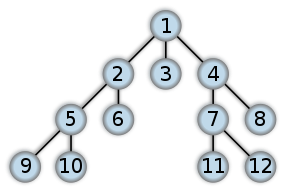
\includegraphics[width=6 cm]{asset/bfs.png}
\end{figure}

\end{frame}

\begin{frame}
\frametitle{BFS (lanj.)}

Berdasarkan ilustrasi di atas, dapat kita lihat bahwa node yang dekat dengan node 1 akan dikunjungi terlebih dahulu. Sementara itu, node yang jauh akan dikunjungi terakhir, seperti node 9 dan 11 yang berjarak 3 dengan node 1.
\newline\newline
Setelah mengetahui konsep BFS dan DFS, kita akan mulai mempelajari implementasinya dalam pemrograman. Dalam potongan kode selanjutnya, akan diberikan contoh kode DFS dan BFS pada unweighted graph yang disimpan menggunakan adjacency matrix.
\end{frame}

\begin{frame}[fragile]
\frametitle{Implementasi DFS}
DFS dapat diimplementasikan menggunakan rekursi atau dengan bantuan struktur data stack. Berikut adalah implementasi DFS rekursi\newline
\begin{lstlisting}
integer AdjMatrix[N][N]
boolean flag[N]
set flag = false
flag[1] = true

procedure DFS(integer currNode):
  for i=1 to N
    <@\textcolor{mygreen}{//check apakah ada edge dan belum pernah dikunjungi}@>
    if AdjMatrix[currNode][i]==1 and flag[i]==false
      flag[i] = true
      DFS(i)
end
				
\end{lstlisting}
\end{frame}

\begin{frame}[fragile]
\frametitle{Implementasi DFS (lanj.)}
Berikut adalah potongan kode untuk implementasi DFS menggunakan stack\newline
\begin{lstlisting}
integer AdjMatrix[N][N]
boolean flag[N]
set flag = false
stack <integer> s

s.push(1), flag[1] = true
while s is not empty
  integer currNode = s.top()
  s.pop()
  for i=1 to N
    if AdjMatrix[currNode][i]==1 and flag[i]==false
      flag[i] = true
      s.push(i)
				
\end{lstlisting}
\end{frame}

\begin{frame}[fragile]
\frametitle{Implementasi BFS}
BFS membutuhkan bantuan struktur data queue. Berikut adalah potongan kodenya\newline
\begin{lstlisting}
integer AdjMatrix[N][N]
boolean flag[N]
set flag = false
queue <integer> q

q.push(1), flag[1] = true
while q is not empty
  integer currNode = q.front()
  q.pop()
  for i=1 to N
    if AdjMatrix[currNode][i]==1 and flag[i]==false
      flag[i] = true
      q.push(i)
				
\end{lstlisting}
\end{frame}

\begin{frame}
\frametitle{Contoh Permasalahan}
Pak Dengklek tinggal di kota A. Suatu hari, beliau ingin pergi ke kota B. Terdapat beberapa jalan yang menghubungkan kota-kota dalam negara tempat beliau tinggal. Namun, karena beliau sudah tua, Pak Dengklek ingin melewati jalan seminimal mungkin untuk sampai ke kota B.
\newline\newline
Diberikan keterangan mengenai kota A, kota B, dan jalan-jalan yang terdapat dalam negara Pak Dengklek, outputkan berapa jalan minimal yang beliau harus lewati untuk pergi dari kota A ke kota B!
\end{frame}

\begin{frame}
\frametitle{Pembahasan Permasalahan}
Permasalahan di atas dapat diselesaikan menggunakan BFS. Karena sifat BFS yang menelusuri node per layer, maka dapat disimpulkan bahwa jika suatu node terkunjungi, maka pasti jarak yang ditempuh merupakan jarak terpendek dari node awal. Hal ini berlaku pada unweighted graph yang edgenya tidak memiliki bobot.
\newline\newline
Dengan demikian, permasalahan di atas dapat diselesaikan dengan menggunakan BFS. Pada slide selanjutnya akan diberikan contoh implementasi untuk menyelesaikan permasalahan jarak terpendek tersebut!
\end{frame}

\begin{frame}[fragile]
\frametitle{Implementasi Permasalahan}

\begin{lstlisting}
integer AdjMatrix[N][N] , A , B , jarak = -1
queue < (integer,integer) > q
<@\textcolor{mygreen}{//Queue menyimpan node yang dikunjungi dan jarak dari A}@>
q.push({A,0}), flag[A] = true
while q is not empty
  (integer,integer) currNode = q.front()
  q.pop()
  <@\textcolor{mygreen}{//Cek jika telah sampai di kota B}@>
  if currNode.first == B
    jarak = currNode.second, break
  for i=1 to N
    if AdjMatrix[currNode.first][i]==1 and flag[i]==false
      flag[i] = true
      q.push({i,currNode.second+1})
if jarak!=-1
  print jarak
else
  print 'Tidak dapat ke kota B'		
\end{lstlisting}
\end{frame}

\begin{frame}
\frametitle{Tree}
\foreignTerm{Tree} merupakan bentuk khusus dari graph. Tree merupakan graph yang mana seluruh nodenya terhubung (tidak ada node yang tidak dapat dikunjungi dari node lain) dan tidak terdapat cycle. Oleh karena itu, jumlah edge dalam sebuah tree pasti berjumlah sebanyak node-1.

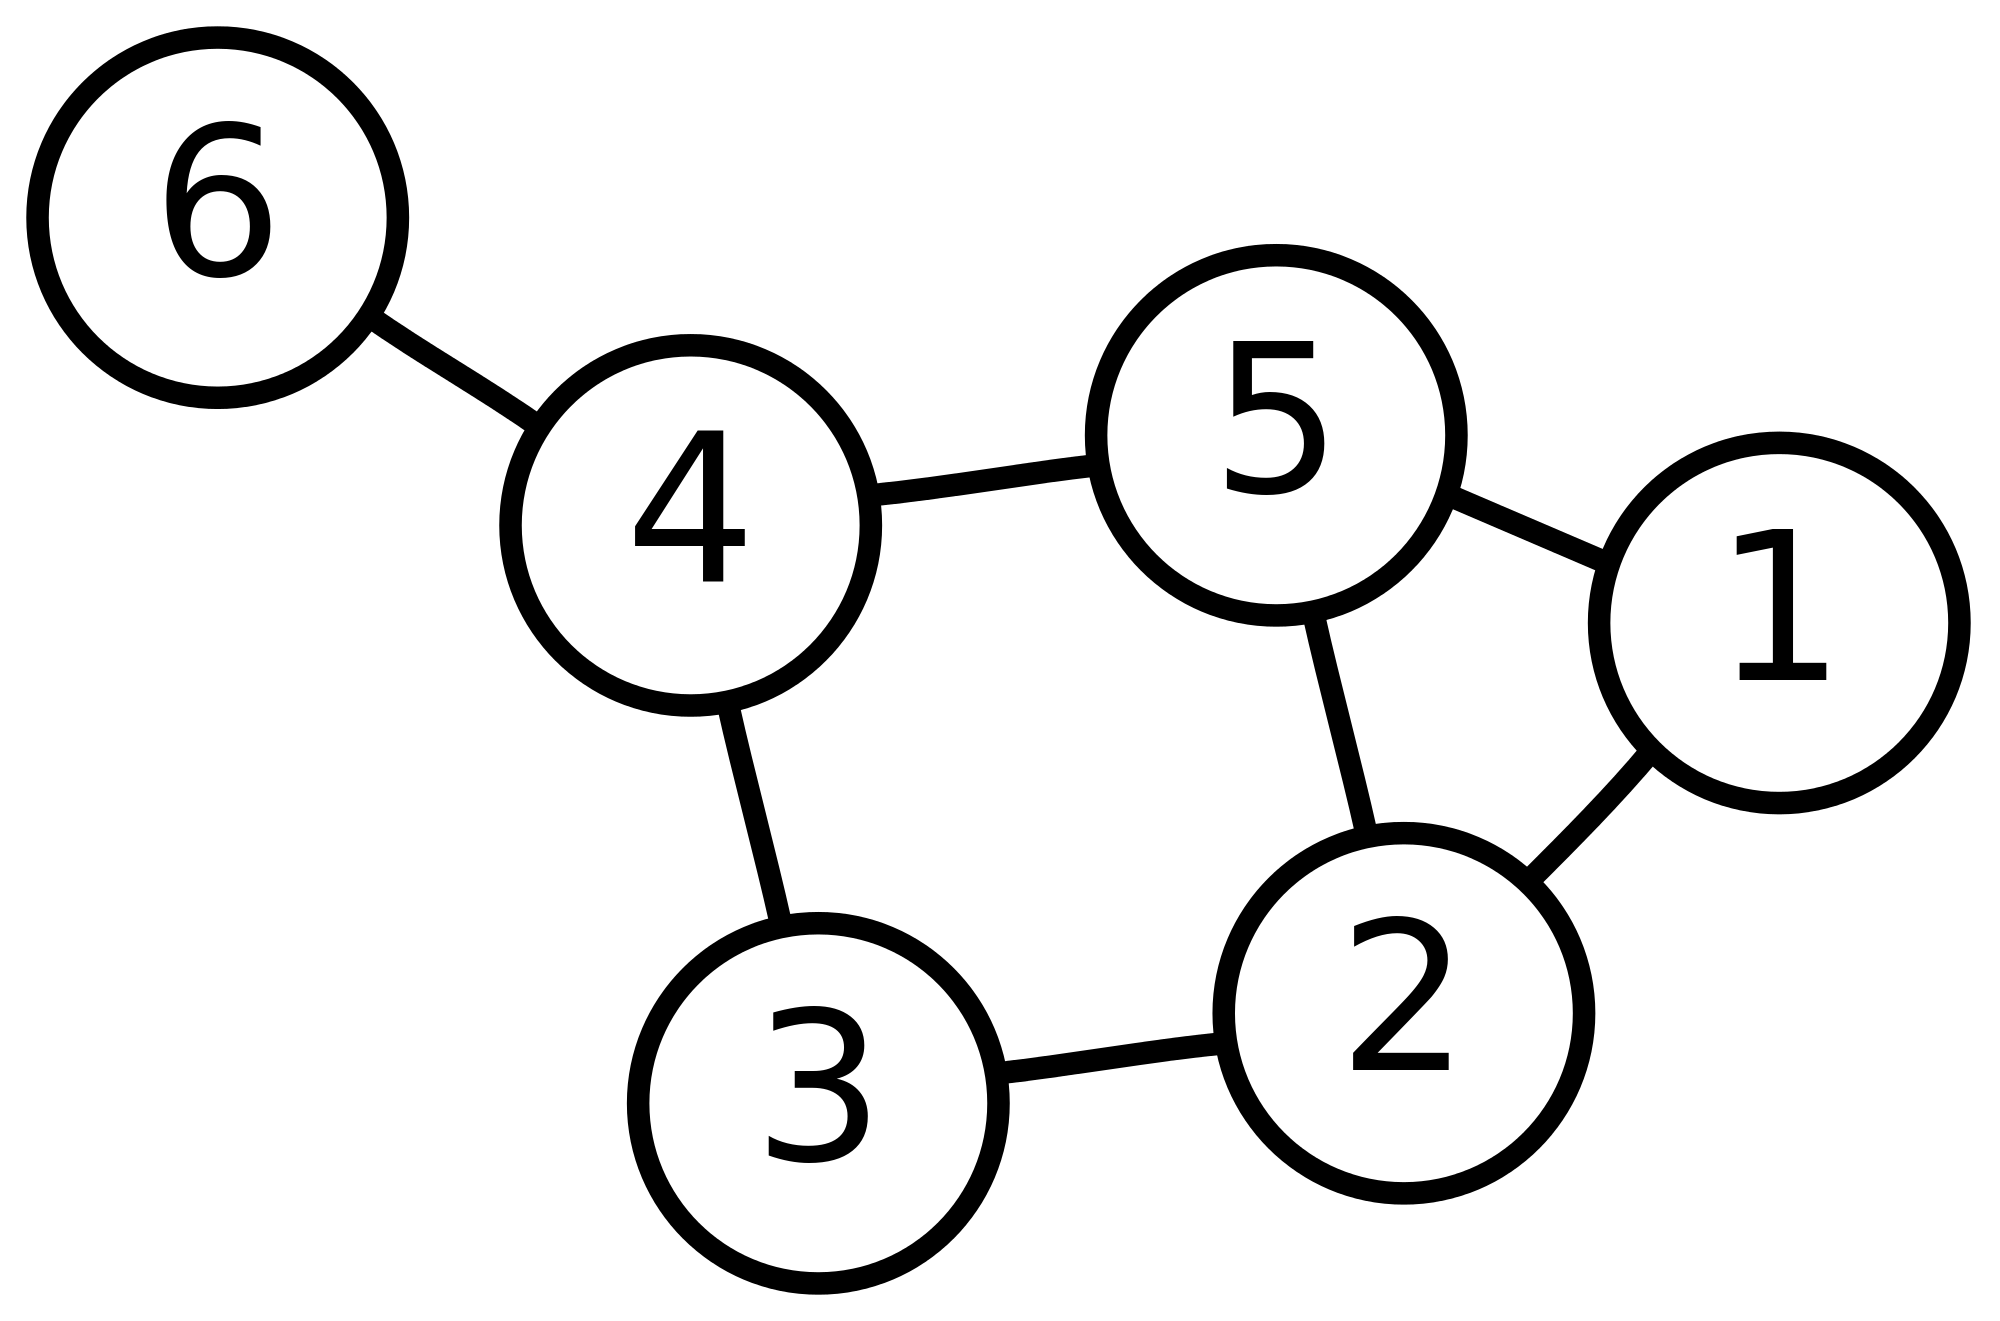
\includegraphics[width=4 cm]{asset/not-tree.png}
\hspace{\fill}
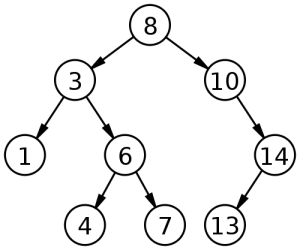
\includegraphics[width=4 cm]{asset/tree.png}
\newline\newline
Pada gambar di atas, gambar kiri bukan sebuah tree karena memiliki cycle, sedangkan gambar kanan merupakan tree. 
\end{frame}

\begin{frame}
\frametitle{Directed Acyclic Graph}
\foreignTerm{Directed Acyclic Graph (DAG)} merupakan bentuk khusus dari directed graph. DAG tidak memiliki direct cycle. Berbeda dengan tree dimana setiap node pasti dapat mencapai node lainnya, sifat tersebut tidak berlaku pada DAG.

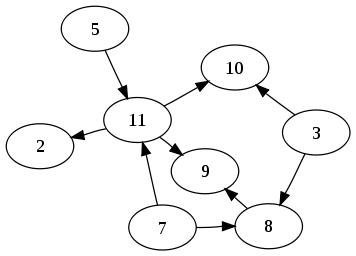
\includegraphics[width=4 cm]{asset/dag.png}
\hspace{\fill}
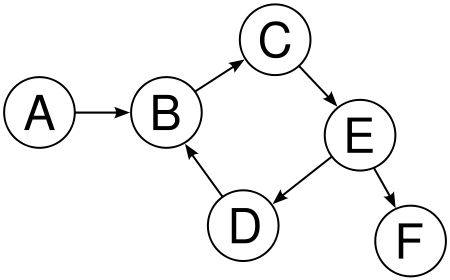
\includegraphics[width=4 cm]{asset/not-dag.png}
\newline\newline
Pada gambar di atas, gambar kiri merupakan DAG, sedangkan gambar kanan bukan DAG karena memiliki cycle
\end{frame}

\end{document}